\documentclass{article}
\usepackage[margin=1.5in]{geometry}
\usepackage{float}
\usepackage{graphicx}
\usepackage{tikz}
\usepackage{pgfplots}
\usepackage{amsmath}
\usepackage{nameref}
\usepackage{siunitx}
\usepackage[utf8]{inputenc}

\newcommand{\cmmnt}[1]{\ignorespaces}
\pgfplotsset{compat=1.13}

\begin{document}

\title{Localization for FRC \\
  \large{A Term Report}
  }
\author{Jinan (Dorothy) Hu, Peter Mitrano, Kacper Puczydlowski, Nicolette Vere}

\maketitle{}

\section{Introduction}

  Knowing the position and orientation of a mobile robot is critical to many tasks. For robots designed for high-speed gameplay, knowing the position and orientation allows the robot to perform complex autonomous behaviors such as shooting and retrieving game objects. In this report, we describe a system for determining the pose $(x, y, \theta)$ of a mobile robot in a cluttered environment. The environment we are interested in is the FIRST Robotics Competition (FRC). FRC is a challenging environment because the robots make rapid and aggressive maneuvers by human drivers for part of the time, and at other times are under complete autonomy. Another challenge is that FRC fields are cluttered with other robots and game pieces such as soccer balls, pool noddles, or inflatable shapes, and these objects change from year to year. A successful localization system for FRC must support up to six robots, as well as occlusion from the playing field elements, unpredictable lighting, and frequent impacts. Our research suggests that there are at least five appropriate methods for localization: cameras and tags, radio and ultrasonic beacons, optical flow, dead reckoning with encoders, and dead reckoning with an IMU. All of these methods have seen success in robot localization.
  
	At the highest level, our project is to allow FRC teams to query the position of their robot on the field. This information is a prerequisite for interesting behaviors such as path following, picking up game pieces, navigating to feeder stations, and detecting slips and collisions. These behaviors are currently beyond the reach of most teams, so we hope that by providing a system for localization, teams can extend our work to these complex behaviors. An important criteria for our system is that it work well not only on the FRC field, but in teams practice spaces. If teams are not confident that their system will perform in competition the same way it performs in their practice spaces, they will not use. The risk is simply too great. This is a challenge that most previous localization systems do not consider. Even though FRC teams do not have a full field to test on, they still need a way to test specific behaviors that are specific to the field. Presently, teams will construct mock-ups of small parts of the field and various game elements to test with. For example, if the game requires shooting basketballs into a hoop, most teams will build or purchase a basketball hoop that is similar to the one used on the field and mount it somewhere in their shop. The important point is that this hoop will be similar but not the same as the hoop on the field, and it will likely be mounted in a slightly different position or orientation. Ideally, using our system teams would be able to use their mock setup as if it were the real field. In other words, teams could test a program that autonomously shoots balls into the hoop in their shop and later use the same code with confidence in the competition. Teams must be able to specify the location of their mock field elements so that our localization system can report position that is relative to this hallucinated version of the field. During competition, when the robot is on the real field, the robot should behave in the same way and with similar or better performance characteristics to when it was in the teams practice space.
	This report begins with a review of existing literature on indoor localization for mobile robots in the \nameref{related_work} section. The strengths and weaknesses of these existing methods are described in the \nameref{methods} section. The \nameref{experiments} section contains information on experiments we conducted. The \nameref{specs} section provides a complete description of our design criteria and system specifications. The \nameref{conclusion} section details our plan moving forward.

\section{Related Work} \label{related_work}

  Robot localization has been studied for decades. Overall, the problem of localizing a mobile robot can be viewed as accurately measure the absolute distance to known landmarks, or by measuring the changes in position over time. All localization methods lie somewhere on a spectrum between these two points of view, and we will henceforth refer to these two ideas as global and local pose estimation. Some of the high level techniques for robot localization are: measuring range at various points around the robot and matching these readings to a map, measuring time of flight or difference of time of arrival to calculate distance to known locations, recognizing landmarks and computing pose relative to those landmarks, and measuring changes in pose and accumulating these changes over time. There are different sensors that can be used for each of these techniques, such as laser range finders, ultrasonic, cameras, inertial measurement units (IMU), encoders, radio, infrared light, visible light, and human-audible sound. Although there are a tremendous number of possible methods for indoor mobile robot localization, there are a few which have received the most attention and shown the most success. These include:
  \begin{itemize}
      \item LIDAR mapping
      \item Ultrasonic mapping
      \item IMU and Encoders fusion
      \item Infrared or Radio and Ultrasonic beacons
      \item Wireless network methods based on signal strength
      \item cameras with visually identifiable tags
      %\item Stereo vision and depth cameras
      \item Optical flow mice and cameras
  \end{itemize}

  In our research, we learned how these techniques work and found descriptions and implementations in order to evaluate them. These descriptions and implementations are presented in this section with the purpose of demonstrating a thorough literature review and of providing background information to the reader.

  \subsection{LIDAR Mapping}
	LIDAR is a sensor that works by measuring the amount of time it takes light to return to the LIDAR after hitting a desired object \cite{keith_LIDAR_2007}. Light travels at about \SI{0.3}{\meter\per\nano\second} which is a constant speed \cite{keith_LIDAR_2007}. The sensor sends a certain amount of beams at certain intervals towards an object. Since light moves at a constant speed the LIDAR can calculate the distance between itself and the object that light was hitting. To calculate distance the formula $\frac{d*c}{2}$ can be used. $d$ is the distance to the object, $c$ is speed of light and then divided by two to account for traveling to the object and back. By repeating this process the LIDAR can produce a map of its surroundings by finding the distance between it and surrounding objects within its detecting range \cite{keith_LIDAR_2007}.
	There is three types of information LIDAR can collect depending on the type of LIDAR. The first is the range to the target which is found topographical LIDAR \cite{keith_LIDAR_2007}. A differential Absorption LIDAR can find the chemical properties of the targets it is measuring. A doppler LIDAR can measure the velocity of a target \cite{keith_LIDAR_2007}. This project would use a topographical LIDAR to measure the distance from itself to other objects to find position.
  Most LIDAR have two main pulse systems for measuring distance. The first system micropulse have lower powered lasers that are usually considered safer \cite{keith_LIDAR_2007}. The wavelength for these is typically 1.0-\SI{1.5}{\meter} \cite{LIDAR_uk_how_2017}. The second system is high energy which have stronger lasers and are typically only used for atmospheric measurements \cite{keith_LIDAR_2007}. The wavelength of these is typically 0.5-\SI{0.55}{\meter} \cite{LIDAR_uk_how_2017}.
	LIDAR does localization by using the map it generated of its surrounding and being able to identify landmarks on the map. The LIDAR system will then compare the location of the landmarks to a previously known map. And since the distance between it and those landmarks are known, the LIDAR system can be used to determine its own position \cite{schlichting_vehicle_2016}. Another approach is to match point clouds found on the most recent map produced by the LIDAR to point clouds on the prior map. This has advantages because it does not rely on there being distinguishing features in the environment. But it also takes more time to compute the map since it has to compare more points than a feature to feature map \cite{li_extracting_nodate}.

  \subsection{Ultrasonic Mapping}

    Ultrasonic mapping (often referred to as sonar) was one of the first techniques used for indoor robot localization, and has been explored deeply since the 1980's. The most common approach is to use multiple emitter-receiver pairs placed around the perimeter of the robot, measure the range at each of those points, then localize to a given map of the environment \cite{drumheller_mobile_1987}. Alternately, some systems use one sensor and rotate it around to achieve the same effect \cite{leonard_mobile_1991, drumheller_mobile_1987}. The algorithms for interpreting the measured distances work by first extracting lines, then matching these lines to an existing map. Reported accuracies of the system in \cite{drumheller_mobile_1987} was 1 ft for position, and \ang{10} for angle. In \cite{drumheller_mobile_1987} and \cite{leonard_mobile_1991}, the reported rate of position updates is \SI{1}{\hertz}. Additionally, some methods will explicitly model the uncertainty of the position estimate, or explicitly model the behavior of ultrasonic sensors to ignore unreliable data. A more recent and sophisticated approach to localizing with sonar can be found in \cite{tardos_robust_2002}, in which 24 sonar sensors in conjunction with encoders were used to perform simultaneous localization and mapping. Their experimental results report drifts of \SI{3.9}{\meter} and \ang{21} over the course of \SI{35}{\meter} of travel.

  \subsection{IMUs and Encoders}
    An inertial measurement unit (IMU) is a sensor reporting the forces acting upon an object, the angular rates of change, and surrounding magnetic field. The device typically comprises an accelerometer, gyroscope, and magnetometer which sense the above data respectively. These devices function by detecting Coriolis forces, inertial forces acting in the direction of motion relative to a rotating reference frame. These forces are proportional to the magnitude of the acceleration. These forces may be detected by a simple strain gauge mechanism or object vibrating at a know frequency ( the rate of change of vibration frequency is detected) \cite{barshan_199354}. The premise behind position sensing using this device involves integrating the data with respect to time to calculate position and orientation. This approach was first used in aeronautics to estimate projectile attitude, orientation, and position \cite{agard_1989}. High cost IMU's have been used historically for defense and transportation systems; the quality of the sensor is high and the data is reliable in these applications. An inertial navigation system (INS) often comprises multiple accelerometers, gyroscopes, and magnetometers to estimate orientation and position. Their performance is increased by referencing, or filtering, one sensor to estimate the error from another. Simple double integration of a filtered system using expensive sensors is often sufficient for position tracking applications like ballistics or missile tracking \cite{barshan_199354}.

    In cost-sensitive systems, this methodology is subject to high error rates from accumulation. Because of integration of accelerometer data, the velocity error term grows linearly and position error quadratically. This introduces a need for filtering, sensor fusion, and optimization based approaches.

      Rarely in mobile applications are IMUs the primary position sensor. Odometers and encoders offer relative position sensing because they measure change between distances, but must be provided with a frame of reference. Most odometry-based sensors are updated at a high-frequency, but are subject to high error rates from gear inefficiencies, wheel slippage during normal rotation, and irregularities in data processing \cite{linchevski_addressing_2007}. Complementary filtering, or using multiple, weighted sources of data, is used to obtain an position estimate. Linear quadratic estimation can be used to estimate the position of a object; however, this technique is relatively complex. The algorithm makes a prediction about the current position, taking into account error from the previous measurements. Once the current data is available, the algorithm uses it to correct the parameters it used to make the estimation, provided the data is of high certainty. Known as a Kalman filter, this process uses a known model of the system and assumes errors in the sensors to smoothen the data. Systems can leverage data from a range sensor \cite{teslic_ekf_2011} or indoor positioning systems that use radio frequency signals \cite{marquez_uwb_2017}.

      Cameras, radio beacons, GPS, and similar landmark-based technologies offer global position sensing and have lower accumulated error than local systems discussed above. However, update frequencies are comparatively low, leading to false predictions or periods of unknown position. To compensate for this phenomenon, systems can leverage data streams with higher update frequencies to interpolate between frames. Forster \textit{et al.} describe a visual-inertial navigation system that uses accelerometer and gyroscope data streamed at a high frequency to estimate a pose trajectory between select frames from the camera. Known as keyframes, these camera data are selected to minimize computational requirements while minimizing feature loss. Often, a parallel thread selects appropriate frames. Then, the IMU data are processed into a relative motion constraint. Effectively, this yields a trajectory of position and orientation between camera updates \cite{forster_CDS_15}.

        If the rate at which the position must be updated is lower than the update rate of the data, many values can be processed and used to calculate an approximation within a given time window. Known as preintegration, this technique, instead of filtering the data, combines many data points into a single trajectory estimate. Then, it transforms the data into the navigation frame, allowing for a smoother approximation of system position. This was beneficial in cases where global position data was unavailable for extended periods of time and decreased the computational load of the localization thread \cite{lupton_vian_2012}. Systems like this are effective because camera data is used to correct IMU data on-line when data is available and rarely fails to update the pose estimate between frames. The above work describes an overall CPU time of about 10ms for data processing and real-time execution, although the system update frequency is unknown.

        Leveraging preintegration, systems expanded sensor fusion frameworks with probabilistic terms and models of relationships between sensors. One such approach used a factor-graph to represent system state variables as nodes on a tree and the functional relationship between them as factors (edges). Instead of updating the state each time new data is available, the factor tree updates relevant state variables add into account an error term \cite{indelman_ifns_2013}. A key aspect of this system relies on frame transformations between sensor data happening at a low level. This takes workload off of the main CPU by utilizing FPGAs or other processors to monitor and process odometry or IMU data \cite{li_gyro_2017}. Implementations of such systems claim reduced computational load and similar performance to ORB-SLAM and other modern navigation systems.

    \begin{figure}[H]
      \centering
      \scalebox{.4}{
      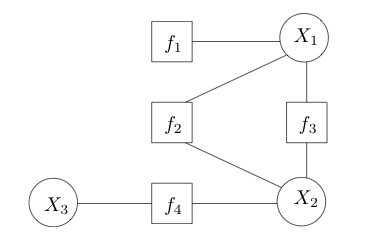
\includegraphics[width=1\linewidth]{./images/Factorgraph.jpg}}
      \label{fig:ex_factor_graph}
      \caption{A simple factor graph \cite{hwymeers_example}.}
    \end{figure}

      Designed for the FIRST Robotics Challenge, frameworks such as Sensor Fusion 2 (SF2) provide users with algorithms for an integrated platform. Some examples are latency correction between IMU and camera data, fusion of encoder and IMU data, and keyframe-based state estimation. Again, these algorithms use known system parameters, such as update frequencies of sensors, frame transformations between sensors, and data from landmarks for filtering and position estimation. Usually, the IMU data is available at a rate an order of magnitude larger than that of the camera. Additionally, the data is accurately timestamped and easily accessible to the vision processing thread. This way, the user receives an updated pose estimate without lag and has an history of the orientation. This is useful for trajectory planning or on-line path correction (like recovering from a collision). Within the next several years, systems like this will mature, offering localization or possibly SLAM.

  \subsection{Beacon systems and Wireless Networks}

    Beacon systems have been used many times with success in the literature. Generally, these systems use ultrasound and or radio as a medium and either signal strength, phase shift, or time to measure distance to the beacons. Among radio systems, the system in \cite{bahl_radar:_2000} identified the location of people moving around buildings using signal strength in the 2.4gHz band received at three or more beacons, and they report accuracy of a few meters with an update rate of at most four times per second. The systems described in \cite{digiampaolo_mobile_2014} uses passive RFID tags on the ceiling and an RFID transmitter on the robot, and report an accuracy of 4\si{\centi\meter} within a 5\si{\square\meter}. Another RFID system \cite{saab_standalone_2011} also uses signal strength to RFID, and reports accuracies for various configurations ranging from 1\si{\centi\meter} to 3\si{\meter}. These RFID systems use readers that cost over \$500.

    There are also countless localization systems that use standard wireless networks. A comprehensive survey of these systems can be found in \cite{liu_survey_2007}. Systems that use signal strength in standard wireless LAN networks have achieved up to 10\si{\centi\meter} accuracy and hundreds of updates per second. Another radio beacon solution is to substitute single-frequency radio with Ultra-wideband radio. These systems can achieve centimeter level accuracy, but they use obscure or custom made transmitters and receivers that cost in the hundreds of dollars \cite{noauthor_dart_nodate} \cite{noauthor_pozyx_nodate}.

    Among ultrasonic beacon systems, \cite{kleeman_optimal_1992} uses the raw arrival times of ultrasonic pulses over time plus odometry together in a Kalman filter. Many beacon systems use the speed difference between sound and electromagnetic waves to measure system. Systems like \cite{smith_tracking_2004}, \cite{ward_new_1997}, and \cite{kim_advanced_2008} send radio pulses followed by ultrasonic pulses. Nodes in the network us the difference in arrival time of these two signals to measure distance. Alternately, some systems use infrared pulses in place of radio \cite{ghidary_new_1999} \cite{yucel_development_2012}. These systems are inexpensive, and report accuracy of between \SI{2}{\centi\meter} and \SI{14}{\centi\meter}.

  \subsection{Cameras with Visual Tags}
		Vision based localization is widely used in robotics. Different visual approaches have been applied to mobile robot systems. Most of vision based systems have cameras on the robots and had either natural landmarks or artificial landmarks in the environments as references to absolute positions. If the natural landmark approach is used, knowing the absolute positions of objects in the circumstance, a robot could calculate its absolute position by calculating orientation and distance toward the object detected and recognized with its absolute position. Another similar approach is using 3D models and 2D to 3D matching techniques. The system described in \cite{sattler_fast_2011} had accurately localized the camera's position using this 2D to 3D mapping technique. Among all of the vision based approaches, the usage of a combination of cameras and artificial landmarks to localize robots is one of the most popular. Common artificial landmarks include 1D binary barcode, 2D binary barcode and 2D colored barcode. The system in \cite{lin_localization_2004} applied the approach of using cameras and ID tags. The system had ID tags on the ceiling, which were \SI{2}{\meter} away from the floor. A web camera,facing to the ceiling, was mounted on a moving robot with a speed of \SI{20}{\centi\meter\per\second}. This system measured the position and orientation of the robot relative to the ID tags through image processing. The result of the experiment in \cite{lin_localization_2004} showed that this method was accurate even though there was an unevenness between the ceiling and the floor. Another system \cite{huh_mobile_2007} also used camera and tags. However, instead of sticking ID tags on the ceiling, it put invisible tags on the floor by every \SI{3.75}{\centi\meter}. The camera it used was surrounded by a UV light, which allowed the camera to capture those invisible tags. This system performed really well in homelike environments, it only had few centimeters of error. Another barcode based localization system of low capacity mobile robot (8 KB memory, 16 MIPs) \cite{dias_barcode-based_2012} used 1d barcodes as references. Using a camera with 80 vertical pixels and 640 horizontal pixels, the system achieved localization within \SI{3.5}{\meter\per\second\square} of error on average. An experiment on 2D barcode based localization was performed on a Pioneer 3 - AT robot. The robot was placed in a random location in the environment and had a Canon VC-C50i analog camera connected with a \SI{1.8}{\giga\hertz} processor and worked under Linux operating System. The robot moved with a speed of \SI{50}{\milli\meter\per\second}, trying to locate itself by finding a code vertically mounted on a wall. The code contained information about its xyz position, normal vectors and its length, therefore, the system would not need to query through databases to find information, which made the process faster.

%   \subsection{Stereo Vision and Depth Cameras}
% We didn't do any background research on this, but we should have so we will do that in B term

  \subsection{Optical Flow}

  % talk about optical flow mice!

	Optical flow is the ability to track changes between cameras frames and measure the differences within them to track position. In other words, optical flow is where given a sequence of images it can find the movement of objects between the images. More exactly optical flow looks at the movement of pixels among images. There are many assumptions about the image that has to be made in order to calculate in order to calculate optical flow. The first is that the lighting in the image stays consistent throughout the sequence of images. Images with inconsistent lighting or transparent objects would violate this assumption. Limiting the amount of inconsistencies in each sequence of images leads to more accurate optical flow.
    
	There are many methods of calculating optical flow that deal with different constraints. This first is the Horn and Schunk method which calculates optical flow looking at all pixels in an image making it considered a global method. Along with the lighting constraint it also adds that the image should be as smooth as possible and have few variations in its coloration. The closer the amount of variations is to zero the more accurate the optical calculation will be\cite{odonovan_optical_2005}.
    
	The optical flow vector for each pixel is calculated using the equation below. $I_x$  and $I_y$  are the spatial gradient of the current pixel. Spatial gradients refer to the the path the pixel is moving along. $I_t$ is the temporal gradient of the current pixel. Temporal gradient is how similar the motion of the pixel is to its neighbors \cite{sun_optical_nodate}. $\alpha$ is a weighting term. $\bar{u}$ and $\bar{v}$ are the components of the average optical flow vector of neighboring pixels. The equation is shown below \ref{eq:hotnandschunk} \cite{odonovan_optical_2005}. $n$ represents which iteration the optical flow calculation is on. Each current pixels optical flow is calculated based on previous iterations pixels. Optical flow calculation will iterate from pixel to pixel until it has calculated optical flow for each pixel.

      \begin{figure}[H]
        \centering
        \begin{equation}
          \begin{split}
            u^{n+1} &= \bar{u}^n-\frac{I_x[I_x\bar{u}^n+I_y\bar{v}^n+I_t]}{\alpha^2+I_x^2+I_y^2} \\
            v^{n+1} &= \bar{v}^n-\frac{I_x[I_y\bar{u}^n+I_y\bar{v}^n+I_t]}{\alpha^2+I_x^2+I_y^2} \\
          \end{split}
        \end{equation}
        \caption{Horn and Schunk Optical Flow vector equation}
        \label{eq:hotnandschunk}
      \end{figure}

  Optical flow can also be done locally using the Lucas Kanade method \cite{sun_optical_nodate}. This methods is based off of the assumption that the optical flow vector of pixels are similar to their surrounding pixels. This method finds optical flow vectors that are consistent with its neighboring pixels' temporal gradients and spatial gradients. Each neighbor is then given a weight based off of how close it is to the pixel. The farther away a pixel is, the lower a weight it is assigned. This is because spatial and temporal gradients are based on how far away a pixel is so the error will be larger. Having a lower weight will reduce the error. The formula for the optical flow vector is a least squares equation shown below in equation \ref{eq:lucaskanade} \cite{odonovan_optical_2005}.

      \begin{figure}[H]
        \centering
        \begin{equation}
          \begin{split}
            E_v &= \sum_{p\in\Omega}W^2(p)[\nabla I(p)\cdot v + I_t(p)] \\
          \end{split}
        \end{equation}
        \caption{Lucas Kanade Optical Flow vector equation}
        \label{eq:lucaskanade}
      \end{figure}


    $\nabla I(p)$ and $I_t(p)$ are the spatial gradient and the temporal gradient for each of the neighboring pixels $p$. $v$ is the optical flow vector for pixel located at $(x, y)$ on the image. $W(p)$ is the weight assigned for each pixel. Local methods tend to work better since they do not allow information about vectors to spread to unrelated regions of the image. This issue of information spreading to unrelated areas of the image is especially problematic in global methods when the assumptions about consistent smoothness and illumination are not fully met. There are a variety of other optical flow methods that focus on different ways of comparing pixels within images but local and global are the most popular methods \cite{odonovan_optical_2005}.

	Lucas Kanade looks at pixels which have a certain pixels that have a large gradient in intensity of color. It changes images to be gray scaled in order to see changes in darkness instead of colors. Lucas Kanade method works the best when it uses pixels that have three certain qualities. The first is that the pixels in a small area have the same brightness. Even though the location of the pixel has changed the brightness is consistent, so using a pixel from that area to track is optimal. They also should be temporally similar meaning the path the pixel takes should change gradually. Pixels should also be spatially similar, meaning that neighboring pixels should have similar motion to each other. Picking pixels that fit these requirements work best with Lucas Kanade \cite{sun_optical_nodate}.

\section{Evaluation of Localization Techniques} \label{methods}

  Each of the techniques presented thus far have strengths and weaknesses. In cases where those strengths and weaknesses are orthogonal, combining multiple techniques improves the overall performance. This is the fundamental principle behind sensor fusion. For example, in \cite{kim_advanced_2008} the authors use a compass to make up for the inability of beacons to measure orientation of the robot. In order to tackle all of the diverse challenges of localization in the FRC environment, we believe it is necessary to combine techniques. In this section we will explain which techniques we have selected for our system and which we have ruled out. We will justify why none of the techniques discussed are sufficient on their own, and explain which the techniques we have chosen work well together.
  
  As stated in section \ref{related_work}, techniques for localization include LIDAR mapping, ultrasonic mapping, IMU and encoders, infrared or radio and ultrasonic beacons, wireless network methods, cameras with tags, and optical flow. Each of these techniques has been used successfully in their respective applications, but not all of them are appropriate for this project.
  
  LIDAR has been shown to be one of the highest performing localization methods in terms of accuracy, precision and update rate. The two reasons why we are not pursuing it further are because it is too expensive and because it requires a boundary to map. LIDARs capable of ranging across an entire FRC field are over \$400, which is the cost limit for any single part on an FRC robot. Additionally, LIDAR techniques also require either mapping on the fly, or an existing map. Mapping on the fly presents its own challenges, and usually suffers from very bad localization for some initial period of time while the map is built. Therefore, a map would have to be provided for the environment. Existing maps would work very well on the competition FRC fields, but would not apply in the practice spaces teams us, and it is unrealistic to have a consistent practice space in an FRC shop.
  
  Ultrasonic mapping has this same issue. Both LIDAR and ultrasonic mapping would work best if teams to place walls up to create a ``pen'' for the robot of known geometry to use as a map, and for this reason we believe LIDAR and ultrasonic mapping are unfit. Another major issue with ultrasonic mapping is the interference between robots. If multiple robots range ultrasonic near one another, there could be cross talk or interference between the signals. For is reason enough to rule out any use of reflecting ultrasonic. Note however that ultrasonic beacons do not have this weakness, since the pulses being emitted are not expected to reflect.

  IMUs within the budget of FRC teams suffer from accumulated drift, and as such they cannot be used in isolation. On the other hand, many FRC students have experience with them, so it would be wise to support basic features such as heading detection and filtering using IMUs. IMUs also complete other localization techniques very well. For example, cameras suffer from the jitter of the robot moving, and encoders fail when the wheels slip. IMUs on the other hand are excellent at detecting jitter and slippage. In this way, an IMU is a good complement to cameras and encoders. Research suggests that a system integrating encoder data with an INS can offer pose tracking within 10\% error on a trajectory of several meters \cite{kacper_cite_this}.
  
  Radio and ultrasonic beacons are very attractive because of their low cost and ability to automatically locate each other. The cost of each beacon, according to the specifications laid out in section \ref{section:system_spec}, are projected to cost about \$30 (see \ref{table:beacon_bom}). Furthermore, Beacons have more flexibility in their placement than tags because they are much smaller and do not need to be on flat surfaces, or in specific orientations. Finally, because each beacon can operate as a transmitter or a receiver, beacons can automatically locate each other which means students will not have to measure their positions or worry about them moving. A procedure for this self-localization is described in section \ref{section:beacon_self_localization}. Beacons also make up for some flaws in the other techniques. Beacons provide absolute global position but updates slowly, which nicely complements IMU and encoder methods which are fast but only measure changes in position. Additionally, beacons are more resistant to jitter than cameras. Finally, by placing the beacons and cameras in different locations we can minimize the effect of occlusion.

  Wireless network systems are among the most popular for indoor localization. However, they also require knowledge and control over the 2.5 gHz spectrum in the area where they are used. At FRC events, there can be dozens of wireless networks running, as well as the wireless networks used on the field for communication between robots. For this reason, we feel that techniques using wireless frequency have too many unknown variables.

  Among the vision based localization systems discussed in the Literature review, there are system that use natural landmarks (object detection) and those that use artificial landmarks (tags). Tag based systems are preferred because they are inexpensive and easy to implement. Natural landmark detection would not perform well because the field of FRC changes over time and dynamic robots are moving all around the field during the competition. Furthermore, implementing real time object recognition is computationally intensive. Among systems using artificial landmarks, not a lot of robot localization system use 1D barcodes as references. A 1D barcode can only contains up to 25 characters, which limits the length of information. Among 2D barcodes, fiducial tags and QR tags are two of most popular choices in mobile robot localization. The advantages and disadvantages of different types (QR, Data matrix, PDF417, fiducial tag) of 2D barcodes are discussed here. QR codes are designed to align with the camera. It contains 268 pixels without payloads. Data Matrix codes are very similar to QR codes, and they have high fault tolerance and fast readability. Data Matrix can be recognized with up to 60\% of the code unrecognizable. PDF417 is famous for a storage of huge amount of data. Complex information such as photographs, signatures can be inserted into PDF417 easily. Fiducial tags contain less information than QR codes. However, many of them can easily be detected in one shot and the process speed for fiducial tags is faster than of QR codes. One of the most commonly used 2D barcode in robotics is fiducial tag. A system in \cite{wang_apriltag_2016} measured the distance between AprilTags and the camera. A sheet of \SI{16.7}{\centi\meter} AprilTags were tested from \SI {0.5}{\meter} to \SI{7}{\meter} away. The calculated distance was almost the same as the real distance from \SI{0.5}{\meter} to \SI{6.5}{\meter}. The position errors were within \SI{0.1}{\meter} from range 0 to \SI{10}{\meter}. However, orientation errors were pretty high (\ang{1.5} off) when the off - axis angle was small, but were within 1 degree from \ang{20} to \ang{75} of off - axis angle. The detected rates for tags were 100\% from 0 to \SI{17}{\meter} away. This system showed that the combination of camera and fiducial tags can potentially localize robots accurately and precisely. The research, \cite{chen_two-stage_2013} developed an algorithm to enhance the quality of QR codes captured in order to improve the recognition rate. Its algorithm successfully recognized 96\% of QR codes under a variety of qualities captured by a mobile phone camera. The average time for decoding a QR code is \SI{593}{\milli\second}. Another deblurring method in \cite{xu_2d_2011} can be applied to enhance the quality of motion-blurred ArUco code.
  Another benefit of cameras with tags is that they provide global position information without much setup or infrastructure. However, camera based systems suffer from occlusion and jitter. They are also generally computationally intensive. These disadvantages can be mitigated with our other localization techniques. In summary, tag based camera systems have been shown to be very accurate and we will incorporate them into our system. 

  Optical flow offers accurate angle measurements and fast updates that are relative to our current position. Like all camera based solutions, the vibration of the robot will likely makes this technique difficult. However, cameras are the most widely used sensor according to our survey of FRC students and alumni, which is another benefit of optical flow and tag based solutions. Optical flow can be applied either to cameras facing the environment or pointed down at the floor.
  The latter is the method used by computer mice, which have optical flow chips designed for high speed motion. Optical flow chips are made for optical flow detection with a specific lenses and microprocessor to get position \cite{font_characterization_2011-1}. These types of chips are built into computer mice with lenses that work only when the mouse is against a flat surface at a specific height from the table. This would be a problem in FRC since the field is not perfectly flat and there are sometimes obstacles that the robots need to drive over. There are also different drive trains which can shift center of balance between sets of wheels which would also cause the mouse to be off the ground. One of the benefits of using a mouse would the fast update rate. Optical flow mice update at 2,000 to 6,469 frames per second according to the ADNS-3080 optical flow sensors specifications \cite{noauthor_sensors_nodate}. They process frames quickly and most teams have mice of some sort they could use. However, a drawback of optical flow mice is their inability to detect rotation. Built into the sensors on mice are ways to ignore rotation since computer users want translation of the mouse to be measure over rotation in order to navigate a computer screen. Lighting is also important to for the camera to be able to clearly pick up images so having a source of light illuminating around the optical flow mouse would also be necessary for teams in order to get the best results \cite{font_characterization_2011-1}.
  
  The other option for optical flow is to use a camera which can be facing in any direction. OpenCV provides libraries and sample programs for running dense optical flow and sparse optical flow. The Lucas-Kanade method of sparse optical flow finds the best points on a frame and tracks the motion of only those points by comparing it to the motion of the pixels around that point. It is assumed all pixels around a point will have similar motion. Dense optical flow tracks the motion of all of the points on frames. Dense optical flow takes longer since it is using all of the points on a frame but can be more accurate \cite{noauthor_OpenCV:_nodate}. In general, optical flow is not sufficient on its own because it does not provide global position information. However, it nicely complements our other systems because it uses a sensor we already plan to use, and provides a source of local position updates not based on any assumptions about wheels or robot dynamics.

  Ultimately, we have identified IMUs, encoders, cameras with tags, beacons, and optical as promising techniques for localization in FRC. These techniques together provide redundant sources of both local and global pose estimates, and account for many of the challenges associated with localization for FRC. We believe that implementing each of these techniques and combining their results will produce a more robust localization than exploring any one of them in depth.

\section{Experimental Results} \label{experiments}

  \subsection{IMU Experiments}
    Using a Kobuki Turtlebot\texttrademark indoor robot platform and the NavX\texttrademark IMU, a state space model of the system will be developed and used for basic relative localization. From previous experimentation with the NavX, the drift rate over a period of several minutes can be up to \ang{1}. The results will be compared against the \texttt{robot\_pose\_ekf} ROS package which offers similar functionality. An experiment was designed to obtain information characterizing the error of the IMU and gyroscope, but could not be completed prior to the completion of this report due to constrains on time. The NavX INS will be placed in an area free from sources of vibration. The IMU will collect timestamped data at several fixed frequencies over several hours. The purpose of this is to obtain information about the static error in the system and characterize it using time and frequency domain features. Additionally, the system will be tested for drift in update frequency which may cause errors in sensor integration.

  \subsection{Measuring Beacon Delays}

      The beacon system relies on measuring the time it takes for a sound signal to travel from the beacons to the robot. To do this accurately, one must account for transmit and receive delays in addition to the actual time of flight. Figure \ref{fig:rx_tx_timing} illustrates the various delays we need to account for. We conducted experiments to get initial estimates of these delays. First, to get an estimate of the radio transmit receive delay, a transmitter and receiver were set up on two microcontrollers. The transmitter sent \SI{5}{\milli\second} pulses of radio energy (no encoded data) every \SI{55}{\milli\second}, and oscilloscope probes were attached to the input pin on the transmitter and the output pin on the receiver. By comparing the time difference between the input and output signals on the oscilloscope, we can determine the total time. Furthermore, we can measure the distance between the transmitter and receiver and subtract from the total time the theoretical time of flight of the radio signal. The full data for these measurements are available in \nameref{appendix:rf-rx-tx}, and an example measurement is shown in figure \ref{fig:rf_delay_ex}. The time of flight of radio over distances of a new centimeters or meters is on the order of nanoseconds. We measured an average delay of \SI{45.175}{\micro\second}, which we attribute to the internal circuitry of the transmitter and receiver. The variance of this delay was \SI{16}{\micro\second}. However, we also measured delays as low as \SI{32}{\micro\second} and as high as \SI{79}{\micro\second}. Since the theoretical time of flight over the distances used in this experiment were at most \SI{1}{\nano\second}, we can conclude that there is both delay and significant variance in the delay of the transmitters and receivers. This information will be used to better model the timing of our beacons to make the system as accurate as possible.

      \begin{figure}
        \centering
        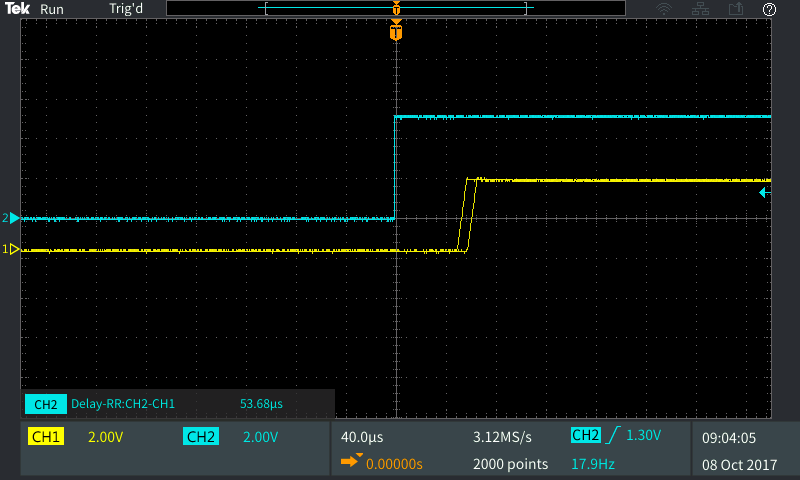
\includegraphics[scale=0.2]{./images/rf_delay_ex.PNG}
        \caption{Example measurement total trip time for radio signal. The blue line is the input to the transmitter, and the yellow is the output of the receiver}
        \label{fig:rf_delay_ex}
      \end{figure}


      Next we performed a similar experiment with the ultrasonic transducers. For this experiment, we used two NTX-1004PZ piezo tweeters placed \SI{25}{\centi\meter} apart. The NTX-1004PZ is meant to be a high-frequency speaker for DJ equipment, and is designed to operate between \SI{4}{\kilo\hertz} and \SI{20}{\kilo\hertz}. However, because they are incredibly cheap we decided to evaluate them as ultrasonic speakers running just above that range. One was connected to a PSoC 5LP for transmitting, and the other was connected only to the oscilloscope. The other oscilloscope prove was connected to the transmitting piezo. The time difference between the transmitting signal on and the receiving signal was measured. The signal applied to the transmitter was short bursts of a 24kHz square wave. The measure time delay between the transmit and receive very closely matched the expected time for sound to travel between the speakers. This indicates that we will not need to account for constant delays in the transmit or receive circuits. However, there were several other noteworthy behaviors we discovered during these tests. First, we noticed that any immediate changes in the frequency of the transmit signal will clicks in the audible range. these clicks do not effect the distance measurement, but they are mildly annoying and should be suppressed if possible by changing the transmit signal.

  \subsection{Measuring Frequency Response}

      After testing for delays in the ultrasonic circuitry, we also measured the frequency response of the NTX-1004PZ. We placed two tweeters in the same configuration as described above. Using a function generator, we transmitted a square wave at 8vPP and swept from \SI{20}{\kilo\hertz} to \SI{30}{\kilo\hertz} and back down over the course of 20 seconds. We attached an oscilloscope to the receiving speaker and captured the power at each frequency using the FFT mode, persisting the display over the course of the sweep to see how the frequency response changes across our frequency range. Figure \ref{fig:frequency_response} shows the results of this experiment. From this experiment, we learned that the best frequency response is achieved at \SI{22}{\kilo\hertz}, and the after \SI{27}{\kilo\hertz} the signal is indistinguishable from the noise.

      \begin{figure}[H]
        \centering
        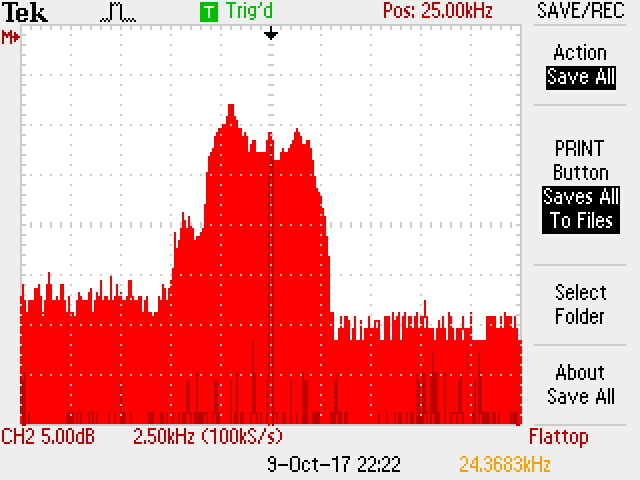
\includegraphics[scale=0.75]{./images/frequency_response.JPG}
        \caption{Frequency response of the NTX-1004PZ. The best response is achieved at 22kHz, and the highest detectable frequency is 27kHz.}
        \label{fig:frequency_response}
      \end{figure}
      
	\subsection{Optical Flow}
    Preliminary testing has been done using a Microsoft USB camera using the sample code provided for dense optical flow in OpenCV. In the screenshot below it can be see in the window labeled flow that there are a variety of green dots on the screen. These are the points that dense optical flow has identified. There is also a green line which is the motion vector of which way the frames are moving. The middle window labeled HSV flow is adding color to the different points that are currently the best for tracking on the frame. The bottom window labeled glitch is the current frame and previous ones overlaid showing all of the motion that has happened.
      \begin{figure}[H]
        \centering
        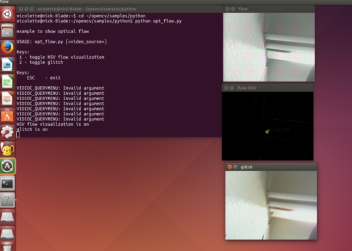
\includegraphics[scale=0.75]{./images/optflow.png}
        \caption{Screenshot of optflow running from OpenCV samples}
        \label{fig:opt_flow}
      \end{figure}
	Testing was then done with the demo for Lucas Kanade based optical flow. Tests were done using lkdemo.cpp which was a sample file provided by OpenCV. Tests were done to see how running this program on a laptop verse the RoboRIO and compare the time they took to run the code. The laptop that the code was run on has a 2.8 GHz Intel 4 Core i7 processor for reference. A chart below was made of the time that each program took to run 100 frames in seconds. 
     \begin{table}[H]
     	\centering
        \label{table:optical_flow_benchmark}
        \begin{tabular}{l|l|l|}
          \cline{2-3}
          & Laptop (s) & RoboRIO (s) \\
          \cline{2-3}
          & 3.638 & 8.429 \\
          & 4.184 & 8.429\\
          & 3.638 & 8.429 \\
          & 3.639 & 8.429 \\
          & 4.184 & 8.429 \\
          \hline
          \multicolumn{1}{|l|}{Average} & 26 & 12 \\
          \hline
        \end{tabular}
        \caption{Time for 100 frames to run using OpenCV on laptop verse RoboRIO}
      \end{table}
	After measuring each 5 times to check for repeatability it can be seen looking at the chart except for the last row how fast in seconds it took for each of the devices to run 100 frames. The last row frames per second was calculated for each device with the laptop reading approximately 26 FPS and the RoboRIO reading 12 FPS. While the laptop was over twice that of the RoboRIO the 12 FPS rate is still fast enough to meet the needs of the project. Other preliminary tests were done with shaking the camera as the program was running after having it initialize the image with marked pixels it had deemed best for measuring. After some shaking of the camera most marked pixels had stayed and only ones that were causes to go off screen by the shaking disappeared. The pixels that the program had decided to measure were based off of what types of pixels work best for Lucas Kanade base optical flow described in the research section of the paper		.

    \subsection{Camera and ArUco Tag}
    	We performed an experiment on clarity of ArUco tags with respect to textures and distance using ArUco tags with a 720p web camera. Six ArUco codes with different IDs were generated by an online ArUco tag generator. These tags have 3 different sizes: \SI{100}{\milli\meter}, \SI{150}{\milli\meter}, \SI{195}{\milli\meter} and 2 different textures: matte, reflective. Those tags were taped together on plywood.
A program using OpenCV ArUco library was ran for 100 frames to count the times of different tags were recognized. For each distance, the program was ran 3 times and the average of the shown up times was calculated. The results of the experiments were shown in the diagram below.

    \begin{figure}[H]
      \centering
      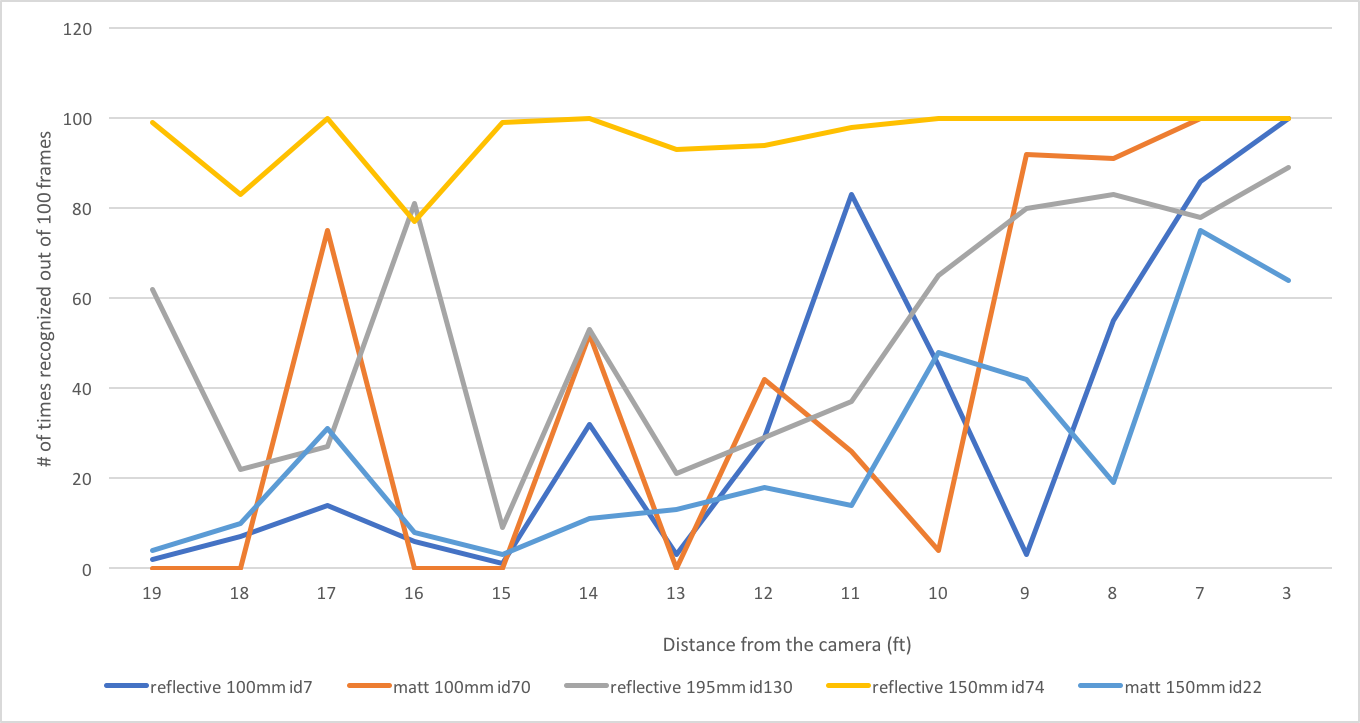
\includegraphics[width = \linewidth]{./images/camera_aterm_experiment.png}
      \caption{Clarity of ArUco tags experiment}
      \label{fig:survey}
    \end{figure}
    There must be other factors other than textures and distances significantly changing the result of this experiment. A similar but improved experiment will be done in the future.
    
\section{System Specification} \label{specs}

  \subsection{Design Criteria}

    Here we present our goals and the criteria our system must meet in order to be successful. Broadly, we consider the following factors to be those which are important to the success of our system.
    \begin{enumerate}
      \item \textbf{Accuracy}\\ how close our position estimates are to ground truth.
      \item \textbf{Precision}\\ how close our position estimates are to each other given the same ground truth.
      \item \textbf{Update Rate}\\ how quickly does our system provide position estimates.
      \item \textbf{Accessibility}\\ how affordable is our system, how difficult is it to make, and how easy is it for teams to use.
    \end{enumerate}

    To come up with hard numbers for these criteria, we first performed a few simple calculations based on our knowledge of FRC. First, we consider what teams would want to use position information for, and decided that the applications requiring the most accuracy are shooting and autonomous pick of game pieces at known locations. Both of these require the position estimates to be close to the true position of the robot. From there, we know that most FRC shooting and pickup mechanisms will work within $\pm$\SI{10}{\centi\meter}. Next, we decided the application requiring the most precision would be path following. If position estimates are imprecise and jump around rapidly, smooth path following will be difficult. From our experience with path following, we estimated that $\pm$\SI{5}{\centi\meter} would be sufficient. For update rate, we considered what the maximum distance a robot could move within a period and used that to decide what our update rate should be. The very fastest FRC robots move \SI{6}{\meter\per\second}, which at an update rate of every \SI{20}{\milli\second} is a distance of $0.02*6 =$ \SI{0.12}{\meter}. The rate of \SI{20}{\milli\second} is a realistic cycle time in FRC, and we feel \SI{12}{\centi\meter} is sufficient given the speed. For accessibility, we acknowledged that teams cannot spend more than \$400 on any part, and that most times source parts from websites AndyMark, Cross-the-road Electronics, and National Instruments among other suppliers. We are also conscious that many FRC teams have limited or cluttered spaces for testing their robots, and may be working in a shared space that must be clean and usable after their work sessions.

    Using all of these informal estimates as a starting point, we conducted a survey of FRC students, Alumni, and mentors. We received 65 responses in total, and used the results of this survey to solidify our design criteria. The full response of this survey are presented in \nameref{appendix:survey}. In summary, the median for accuracy was \SI{10}{\centi\meter} in x,y and \ang{5} in yaw. Our survey did not include questions about precision and update rate, because they depend on what position is used for. Instead, we asked if students would try path planning if they had a localization system, which would back up our estimate of precision. Our survey indicated that 90\% of students would try to make the robot autonomously follow paths. Therefore, our precision estimated based on path planning as an application is supported by our survey. Update rate was not addressed in the survey because we didn't think FRC students would have informed opinions on this metric. Finally, we asked several questions about the accessibility requirements. A cost of under \$200 was deemed acceptable by 84.6\% of responses, and so we have made \$200 our goal for cost. Furthermore, we learned that the amount of space in teams shops varies from a 5 by 5 foot space up to several thousand square feet, but the median shop size is 775 $ft^2$, which one can imagine as a 25 by 30 ft space. In terms of access, about 76.5\% of teams could leave up tags or beacons, with the others stating that they must clean up everything because they work in a shared space such as a classroom. Lastly, we asked students what sensors they were familiar with. The most familiar sensors were cameras (90\%), followed by encoders (84.6\%), then IMUs (60\%). Therefore, it would be beneficial to incorporate cameras, encoders, and IMUs because teams are already familiar with them.

    Ultimately, we formulated design criteria based on our own experience with FRC and with localization, as well as by conducting a survey of the needs, experience, and opinions of FRC participants. These design criteria will help us pick which localization techniques to pursue as well as define the goals for our system.

  \subsection{System Specification}\label{section:system_spec}

    Based on the extensive literature review, the few preliminary experiments we've conducted, and our design criteria, we eliminated our initial list of possible techniques down to the following five:

    \begin{enumerate}
        \item Radio and ultrasonic beacons
        \item IMU
        \item Drive wheel encoders
        \item Optical flow
        \item Camera with matrix tags
    \end{enumerate}

    We have found examples of each of these techniques being used successfully, and in many cases have verified that they satisfy our criteria for accuracy, precision, update rate, and accessibility criteria. We are confident that any combination of these methods would work. These techniques are complementary in their sources of error, and together we believe they will make a robust localization system.

  \subsection{Timeline and Goals}

    To maximize the likelihood that our project is complete in timely manner and with rigorous methodology, we have drafted a set of goals and a timeline to help us manage our time. Below we present our set of \textit{must} goals, which we have agreed are all required for our project to be a success (in no particular order).

    \begin{itemize}
      \item Support 4 wheel differential drive robots moving at continuous driving speeds of up to \SI{3}{\meter\per\second}
      \item Support the NavX and do complementary and basic Kalman filtering
      \item Differentiate between tags with the camera and measure pose relative to them with a standard 720p webcam.
      \item Beacons provide global position updates.
      \item Use the out of the box OpenCV API to get x and y translation between frames
      \item Provide a GUI for specifying the configuration of the sensors on the robot and the configuration of the field or practice space.
      \item Accurately describe the conditions under which camera localization will work, especially with respect to jitter and occlusion.
      \item Support getting the position from each subsystem individually
      \item Support getting one fused position update
      \item Specify what kinds of sensor mounting configurations are supported
      \item Specify which of the subsystems are necessary and which are optional (ex: encoders are necessary, beacons are optional)
      \item Provide the designs and the code for the beacons.
      \item Provide the optimal analysis or coverage of an empty FRC field and the 2018 field
      \item Provide the methodology for finding the optimal placement of tags and beacons for other shape fields
      \item Fail gracefully when some of the sensing techniques are unreliable or failing
    \end{itemize}

    These goals will hopefully constrain the scope of each localization technique such that all of them can be incorporated to some degree. Furthermore, we have drafted a timeline of which of these goals we will focus on over the course of the year. For example, by choosing to start with encoders, IMUs, and cameras, we will be able to have a working localization system even without the other techniques. Additionally, we hope that by giving an end date for some of the components we will be able to move on and not spend too long optimizing any one component.

    \begin{itemize}
      \item B Term:
      \begin{itemize}
        \item Meet goals for encoders, IMUs, and cameras with tags
        \item Specifying robot configuration and tag locations in the GUI
      \end{itemize}
      \item C Term:
      \begin{itemize}
        \item Meet goals for beacons and optical flow
        \item Fuse all techniques into one position update
        \item GUI supports configuring beacons
      \end{itemize}
      \item D Term:
      \begin{itemize}
        \item Meet documentation goals for teams
        \item Provide the designs and the code for all components
        \item Write the final report
      \end{itemize}
    \end{itemize}

  \subsection{Implementation Details}

    Having decided on the sensing techniques we will use, we now describe our detailed system Specification. Ideally, the description in this section serves as the full plan for our implementation of the system during B Term, and most of the major design decisions have been made and clearly presented. 

    \subsubsection{Encoder IMU Fusion}

      The fusion of Encoder and IMU data will be the foundation of our localization system. While we do not plan to explore it too deeply, it will be the first component we work on in B term. The sensors supported will be the Kauai Labs\texttrademark NavX MXP and Micro. The system will not prevent the user from interfacing with either sensor in other ways. The IMU and encoder toolkit will feature an interface for user to input information about their kinematic base, namely wheel radius, wheelbase length, and encoder resolution. Using this information, the system will generate a state space model comprising minimally position and velocity terms. The drivetrain configuration that will be supported is a differential four wheel drive. Support may later be offered for one omnidirectional configuration, such as H-Drive. Using this information, a Kalman and complementary filtering program will be developed. Inputing a sensor configuration in software will allow a team to display local trajectories using a 2-D visualization. The team must be able to quickly modify parameters such as the filtering function used or the radius of a wheel and recalibrate each sensor on-line. This portion of the project must be completed approximately at the start of the FIRST build season.
      
      

      \textbf{Calibration} \\

      \textbf{Description of the Robot Model} \\


    \subsubsection{Radio and Ultrasonic Beacons}

      Important implementation details of the beacon system include the number of beacons needed, the radio communications protocol, and the ultrasonic signal format. The number of beacons can either be picked to minimize cost, and then the beacons can be designed to meet this criteria, or the characteristics of the beacons can be determined and the number of beacons needed derived from that. In order to support arbitrary practice areas, the second method is preferred. In this section we cover relevant calculations and possible implementation details for beacons. \\

      \textbf{Overview of components} \\
      Each beacon consists of a PSoc5 LP processor, NTX-1004PZ piezo transducer, XY-MK \SI{433}{\mega\hertz} radio transmitter, XY-FST \SI{433}{\mega\hertz} radio receiver, and other supporting components. During normal operation, each beacon will listen for a radio signal telling it to emit an ultrasonic signal. We expect that a few other components such as resistors, LEDs, and a battery will be required for the final beacon. \\

      \textbf{Format for Ultrasonic Signal} \\
      The ultrasonic signal should be designed to maximize both the distance it can be detected from and accuracy with which it's timing can be detected. Using a simple pulse of fixed frequency and amplitude is not ideal because it trades off energy transmitted (and thus distance) with accuracy. This is because a longer pulse contained more energy and can be detected from further, but at the same time the receiver cannot distinguish timing within the length of the pulse. Therefore, a chirp signal will be used. Compare the usual function relating amplitude to time of a sine wave to the quadratic chirp signal.
      $$ x(t) = A\cos(\omega t + \phi) $$
      $$ x(t) = A\cos\bigg(2\pi\Big(\tfrac{f_1 - f_0}{2T}t^2+f_0t\Big) + \phi\bigg) $$

      This function will generate a chirp with amplitude $A$, starting from frequency $f_0$ going to $f_1$ over time interval $T$. Figure \ref{fig:chirp} shows the specific waveform with the parameters we expect to use. This is a linear chirp signal because the instantaneous frequency of the signal changes linearly with time.

      \begin{figure}[H]
        \centering
        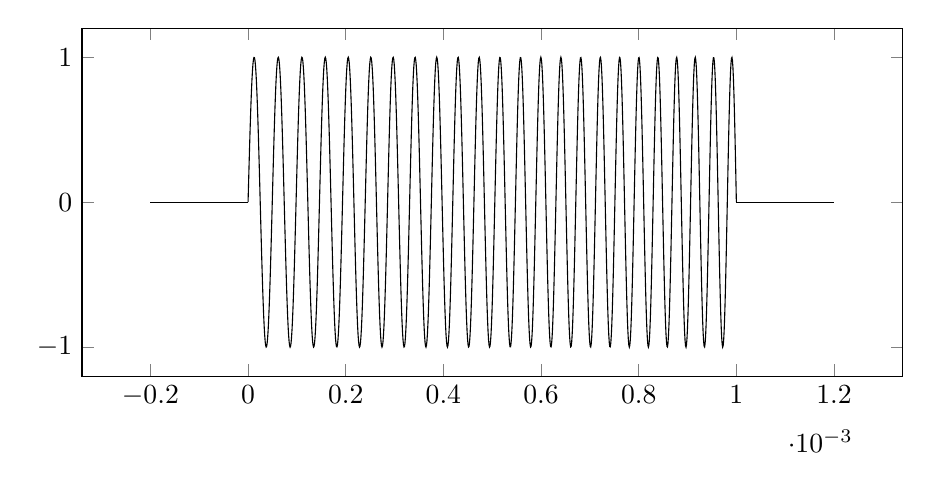
\begin{tikzpicture}
          \begin{axis}[width=12cm,height=6cm]
            \addplot[domain=-.0002:0,samples=10]{0};
            \addplot[domain=0:0.001,samples=1000]{sin((2*180*((27000 - 20000)/(2*0.001)*x*x + 20000*x)))};
            \addplot[domain=0.001:0.0012,samples=10]{0};
          \end{axis}
        \end{tikzpicture}
        \label{fig:chirp}
        \caption{Chirp signal with $\phi=0$, $A=1$, $f_0=\SI{20}{\kilo\hertz}$, $f_1=\SI{27}{\kilo\hertz}$, and $T=\SI{1}{\milli\second}$}
      \end{figure}

        This is the waveform we will be emitting from the ultrasonic sensors. The benefit is that it can be high power and still allow the receiver to determine precisely where in the waveform it is listening. One method for doing this is to take the discrete short time Fourier transform, which will show us how the power at various frequencies changes over time. By applying the FFT at a particular instant during the chirp, we can determine the position in time within the chirp of the current FFT. For instance, in the signal above if we apply and FFT at time $t_n=1.0$ and discover high power at frequency $f=\SI{22}{\kilo\hertz}$, we know that the chirp began at time $t_0 = t_n - \tfrac{f - f_0}{f_1 - f_0}T = 1.0 - \tfrac{22-20}{27-20}0.001 = 0.99857$. Another simpler strategy is to slide the waveform you expect to hear across samples of recorded raw input and check for the point of highest correlation. In other words, slide the waveform in figure \ref{fig:chirp} and match it to the received signal. Both of these techniques are used in practice, and we are considering both in our implementation. \cmmnt{what are the pros and cons}

        Our beacon system relies on accurately knowing the distance to a beacon, and therefore knowing exactly when the start of the signal left the transmitter and when the start of the signal arrived at the receiver. Figure \ref{fig:rx_tx_timing} shows the sources of delay we are accounting for, and we describe our methodology for measuring these delays in the \nameref{experiments} section. \\

      \begin{figure}
        \centering
        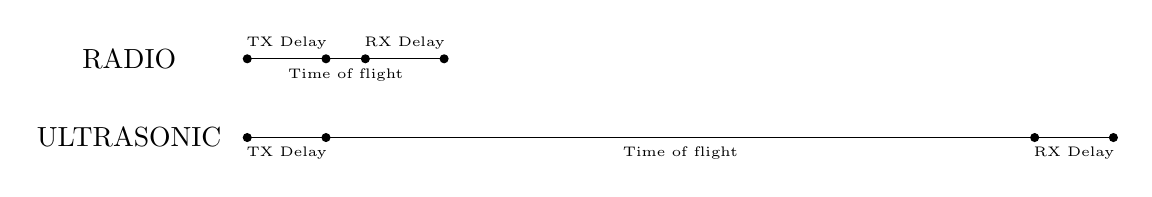
\begin{tikzpicture}
          % timeline for ultrasonic
          \draw (-1.5, 0) node {ULTRASONIC};
          \filldraw (0,0) circle (0.05);
          \draw (0.5, -0.2) node {\tiny TX Delay};
          \draw (0,0) -- (1,0);
          \filldraw (1,0) circle (0.05);
          \draw (5.5, -0.2) node {\tiny Time of flight};
          \draw (1,0) -- (10,0);
          \filldraw (10,0) circle (0.05);
          \draw (10.5, -0.2) node {\tiny RX Delay};
          \draw (10,0) -- (11,0);
          \filldraw (11,0) circle (0.05);

          % timeline for radio
          \draw (-1.5, 1) node {RADIO};
          \filldraw (0,1) circle (0.05);
          \draw (0.5, 1.2) node {\tiny TX Delay};
          \draw (0,1) -- (1,1);
          \filldraw (1,1) circle (0.05);
          \draw (1.25, 0.8) node {\tiny Time of flight};
          \draw (1,1) -- (1.5,1);
          \filldraw (1.5,1) circle (0.05);
          \draw (2.0, 1.2) node {\tiny RX Delay};
          \draw (1.5,1) -- (2.5,1);
          \filldraw (2.5,1) circle (0.05);
        \end{tikzpicture}
        \label{fig:rx_tx_timing}
        \caption{Timing of radio and ultrasonic signals. Experiments indicate \SI{46.175}{\micro\second} total RF delay and \SI{1}{\milli\second} total ultrasonic delay.}
      \end{figure}

      \textbf{Path Loss} \\
      We calculate the free space path loss (FSPL) of the radio signals at the farthest distance from the beacons. For this calculation, we assume the worst case where the beacon is on the other side of the length field, which is $\SI{16.5}{\meter}$ away. Over the more realistic distance of half the width of the field (\SI{5.6}{\meter}), the path loss is only \SI{40}{\decibel}. \\
      $$ \text{FSPL} = 20\log_{10}\Bigg(\frac{4\pi Rf^2}{c^2}\Bigg) = 20\log_{10}\Bigg(\frac{4\pi*16.5*\SI{433e6}{\hertz}}{\SI{3e8}{\meter\per\second}}\Bigg) = 49.521 $$

      \begin{table}
        \label{table:beacon_bom}
        \begin{tabular}{|l|l|}
          \hline
          Item & Cost per Beacon \\
          \hline
          PSoc 5LP & \$10.00 \\
          RF Tx/Rx Pair & \$1.68 \\
          piezo speaker & \$1.65 \\
          9v battery & \$1.19 \\
          battery connector & \$0.54 \\
          LCD display & \$3.90 (optional) \\
          resistors and capacitors & \$5.00 (estimate) \\
          prototyping board & \$5.00 (estimate) \\
          \hline
          Total & 28.96 \\
          \hline
        \end{tabular}
        \caption{estimated bill of material for beacons}
      \end{table}

      \textbf{Self-Localization of Beacons} \label{section:beacon_self_localization}\\
      Beacons that can automatically discover each other and their relative positions will tremendously improve the easy of setup for the beacon system. We believe this is possible, and in this section we describe a protocol for doing so.

      When the first beacon is turned on, it will listen for radio packets for a brief period of time to check if it is the first beacon to be turned on. If it hears nothing, it will assume it is the first beacon and assign itself ID 0. This beacon will be responsible for sending the synchronizing radio pulse as well as handle the distribution of IDs to the other beacons. At this point, beacon 0 will send packets advertising that ID 1 is available. When the next beacon is turned on, it will get the message that ID 1 is available, assign itself that ID, and respond with an ACK message confirming that ID 1 is now taken. Beacon 0 will then begin advertising that ID 2 is available. This process continues for N beacons. Once each beacon has its assigned ID number, beacon 0 will start organizing the self-localization of each beacon. First, beacon 0 will send a packet telling everyone that beacon 0 will transmit ultrasonic. All beacons other than beacon 0 will hear this and start a timer, and beacon 0 will itself transmit ultrasonic. Each beacon will receive this ultrasonic and compute its distance to beacon 0. After waiting a fixed period of time (such as \SI{50}{\milli\second}) for this process to complete, beacon 0 will send a packet telling everyone that beacon 1 will transmit ultrasonic. This process continues until every beacon has recorded its distance to every other beacon. At this point, beacon 0 will tell each beacon sequentially to report its distance calculations to beacon 0. Beacon 0 will then compute the location of every beacons by minimizing the least squares error in the system of equations defining the beacon locations. Finally, it will report the resulting positions to all the beacons. These communications can also be monitors from a laptop with an inexpensive USB software defined radio, such that the status and result of this process can be shown in a GUI and debugging information can be communicated. \\

      \textbf{Number of Beacons Needed} \\
      The number of beacons can be decided once the range and beam pattern of the beacons is known. To do this, a rigorous test that measures the sound level at various angles and distance will be performed. Once this is known, we can offer a tool or set of steps to determine how many beacons are needed and where beacons should be placed.

    \subsubsection{User Interface (GUI)}

      As mentioned above, one of our goals is to develop a GUI. This GUI will serve several functions, such as displaying the position of the robot on the field, showing debug information from each subsystem, and allowing students to input parameters about their robot and their practice space. For example, doing forward kinematics with the encoders requires that the position of each wheel and encoder is known. Additionally, the GUI could allow a visual interface for the students to say where and how their practice space maps to the imaginary FRC field.

\section{Conclusion} \label{conclusion}

  Over the course of A Term, we conducted thorough background research on various methods for localization and evaluated their performance. Based on numerous reports for each localization technique, a survey of FRC students and alumni, and our own knowledge of the challenges of localization for FRC we narrowed down the list of possible techniques to encoders, IMUs, beacons, cameras and tags, and optical flow. Each of these methods has been shown to work in other indoor mobile robot environments, and together they make up for the weakness of each individual method. Our strategy will be to apply each of these five techniques to the degree we believe is necessary to meet our design criteria, rather than to choose one method and optimize it deeply. Our performance will be judged against the design criteria stated above, and we have developed goals and a timeline to guide our work moving forward.

\section{Appendix}

  \subsection{Appendix A}\label{appendix:survey}

    Survey Responses

    \begin{figure}[H]
      %\centering
      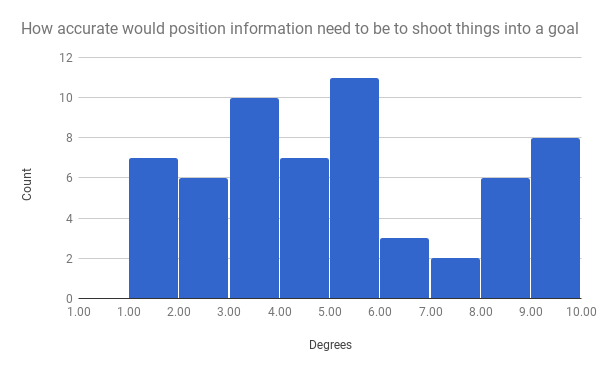
\includegraphics[height=4.2cm]{./images/survey_angle.png}
      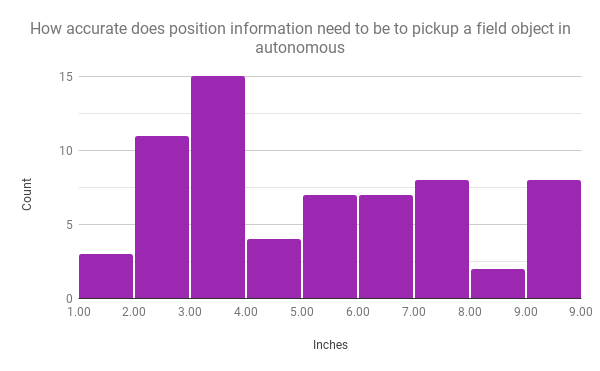
\includegraphics[height=4.2cm]{./images/survey_position.png}
      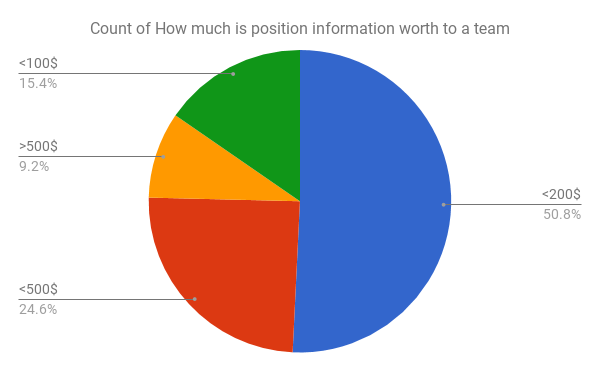
\includegraphics[height=4.2cm]{./images/survey_worth.png}
      \label{fig:survey}
    \end{figure}

  \subsection{Appendix B}\label{appendix:rf-rx-tx}

    \begin{table}[H]
      \begin{tabular}{|l|l|l|l|l|}
        \hline
        Measured Distance (m) & \multicolumn{3}{|l|}{Measured Total Time ($\mu$s)} & Average Delay \\
        \hline
        0.0630 & 45.44 & 42.80 & 34.48 & 40.90646 \\
        0.1425 & 52.72 & 50.48 & 52.09 & 51.76286 \\
        0.1505 & 64.16 & 63.36 & 60.24 & 62.58616 \\
        0.2210 & 40.33 & 36.79 & 36.40 & 37.83926 \\
        0.2415 & 49.52 & 45.76 & 43.92 & 46.39919 \\
        0.2460 & 47.47 & 53.84 & 44.71 & 48.67251 \\
        0.2965 & 34.36 & 34.00 & 43.76 & 37.37234 \\
        0.3085 & 79.36 & 62.16 & 59.52 & 67.01230 \\
        0.3390 & 39.92 & 57.27 & 38.96 & 45.38220 \\
        0.3770 & 41.75 & 40.75 & 45.53 & 42.67541 \\
        0.3600 & 38.40 & 38.40 & 37.68 & 38.15880 \\
        0.0070 & 35.60 & 36.08 & 34.32 & 35.33331 \\
        \hline
        \multicolumn{4}{|r|}{Average Delay ($\mu$s)} & 46.175 \\
        \hline
      \end{tabular}
      \caption{The time of flight of radio over tens of centimeters is insignificant compared to the delay within the transmitter and receiver.}
      \label{table:rf-rx-tx}
    \end{table}

\bibliographystyle{plain}
\bibliography{phil-mqp}
\end{document}
